\documentclass[	DIV=calc,%
							paper=a4,%
							fontsize=9pt,%
							twocolumn]{scrartcl}	 					% KOMA-article class

\usepackage{lipsum}													% Package to create dummy text
\usepackage[english]{babel}										% English language/hyphenation
\usepackage[protrusion=true,expansion=true]{microtype}				% Better typography
\usepackage{amsmath,amsfonts,amsthm}					% Math packages
\usepackage[pdftex]{graphicx}									% Enable pdflatex
\usepackage[svgnames]{xcolor}									% Enabling colors by their 'svgnames'
\usepackage[hang, small,labelfont=bf,up,textfont=it,up]{caption}	% Custom captions under/above floats
\usepackage{epstopdf}												% Converts .eps to .pdf
\usepackage{subfig}													% Subfigures
\usepackage{booktabs}												% Nicer tables
\usepackage{fix-cm}	
\usepackage{color}
\usepackage{hyperref}
\usepackage{amsmath}
\usepackage{amssymb}
\usepackage{tikz}
\usepackage{tabularx}
\usepackage{amsmath}
\usepackage{layouts}
\usepackage{array}
\usepackage{tikz}
\usepackage{amssymb}
\usepackage{graphics}
\usepackage{lmodern}
\usepackage{epstopdf}
\usepackage[T1]{fontenc}
\usepackage[utf8]{inputenc}
\usepackage{authblk}
\usepackage{tabularx}
\usepackage{multirow}
\usepackage{bm}
\usepackage{here}
\usepackage{biblatex} 
\bibliography{report} 
\usepackage{enumerate}
\usepackage{booktabs}	
\usepackage{algorithm}
\usepackage{algorithmic}


%%% Custom sectioning (sectsty package)
\usepackage{sectsty}													% Custom sectioning (see below)
\allsectionsfont{%															% Change font of al section commands
	\usefont{OT1}{phv}{b}{n}%										% bch-b-n: CharterBT-Bold font
	}

\sectionfont{%																% Change font of \section command
	\usefont{OT1}{phv}{b}{n}%										% bch-b-n: CharterBT-Bold font
	}


\hypersetup{
  colorlinks,%
    citecolor=black,%
    filecolor=black,%
    linkcolor=black,%
    urlcolor=black
}

%%% Headers and footers
\usepackage{fancyhdr}												% Needed to define custom headers/footers
	\pagestyle{fancy}														% Enabling the custom headers/footers
\usepackage{lastpage}	

% Header (empty)
\lhead{}
\chead{}
\rhead{}
% Footer (you may change this to your own needs)
\lfoot{\footnotesize \texttt{NAO Localization} \textbullet ~University of Amsterdam}
\cfoot{}
\rfoot{\footnotesize page \thepage\ of \pageref{LastPage}}	% "Page 1 of 2"
\renewcommand{\headrulewidth}{0.0pt}
\renewcommand{\footrulewidth}{0.4pt}



 \newcommand{\tab}{\hspace*{2em}} % tabs for pseudocode indent


%%% Creating an initial of the very first character of the content
\usepackage{lettrine}
\newcommand{\initial}[1]{%
     \lettrine[lines=3,lhang=0.3,nindent=0em]{
     				\color{DarkGoldenrod}
     				{\textsf{#1}}}{}}



%%% Title, author and date metadata
\usepackage{titling}															% For custom titles

\newcommand{\HorRule}{\color{DarkGoldenrod}%			% Creating a horizontal rule
									  	\rule{\linewidth}{1pt}%
										}

\pretitle{\vspace{-30pt} \begin{flushleft} \HorRule 
				\fontsize{25}{25} \usefont{OT1}{phv}{b}{n} \color{DarkRed} \selectfont 
				}
\title{Feature Detection and Localization for the Robocup SPL}					% Title of your article goes here
\posttitle{\par\end{flushleft}\vskip 0.5em}

\preauthor{\begin{flushleft}
					\large \lineskip 0.5em \usefont{OT1}{phv}{b}{sl} \color{DarkRed}}
				
\author{Amogh \textsc{Gudi} {\small\emph{(23408036)}}, Patrick \textsc{de Kok} {\small\emph{(5640318)}},
        Georgios \textsc{K. Methenitis} {\small\emph{(10407537)}},
		Nikolaas \textsc{Steenbergen} {\small\emph{(10333681)}}\\}											% Author name goes here
\postauthor{\footnotesize \usefont{OT1}{phv}{m}{sl} \color{Black} 
					University of Amsterdam 								% Institution of author
					\end{flushleft}\HorRule}

%%% Begin document
\begin{document}
\maketitle
\thispagestyle{fancy} 			% Enabling the custom headers/footers for the first page 
% The first character should be within \initial{}
\initial{I}\textbf{n this project we propose a basic code for the RoboCup Soccer Standard Platform League for the Dutch Nao Team. We focused on the problem of visual feature recognition and the localization of the robot in a tournament setup. This project contains a detailed description of our implementation together with a conclusion and a brief evaluation. Since this report only covers feature detection and localization we give an outlook on what parts are to be implemented in addition to make the robots play soccer.}

\section{Introduction}
\textit{
By mid-21st century, a team of fully autonomous humanoid robot soccer players shall win the soccer game, comply with the official rule of the FIFA, against the winner of the most recent World Cup.}

\hfill -- RoboCup Initiative, objective statement~\cite{RoboCupObjective,kitano1997robocup}

RoboCup encompasses a set of competitions, stimulating innovation and research towards reaching one of the grand challenges within both the robotics and AI community -- defeating the most recent World Cup winning soccer team by a team of robots in 2050.  This demands for systems which can deal with a dynamic environment with a continuous, incompletely observable state space, with non-symbolic sensor readings and with cooperation.

The best known competition of RoboCup is RoboCup Soccer.  This competition encompasses 5 leagues, each with different rules imposed on the game as well as on the participating robots~\cite{RoboCupSTL}.  These differences induce a different research focus within each league.  One of those leagues is the Standard Platform League, where all teams use identical robots.  The Robocup Federation states that ``[t]herefore the teams concentrate on software development only, while still using state-of-the-art robots. Omnidirectional vision is not allowed, forcing decision-making to trade vision resources for self-localization and ball localization.''~\cite{RoboCupSTL}

To keep on pushing research forwards and the community of participating teams motivated to implement and design new methods, the RoboCup Soccer competition updates the rules each year.  One of the more recent updates in the rules is that all goal posts should be yellow, whereas before there were two differently colored goal posts.  This puts an emphasis on the implementation and enhancement of localization algorithms as the field is completely symmetrical.

The Dutch Nao Team has participated since 2010 in the RoboCup Standard Platform League (STL)~\cite{DNT-TD10, DNT-TD11, DNT-TD12} and plans doing so for 2013 as well~\cite{DNT-TD13}.  The software package used during the previous cup has been written in Python.  Its localization algorithm was very heuristic and course-grained; it did not made explicit where the robot was placed, but indicated whether the robot should kick the ball\footnote{The robot would kick the ball in the direction of a goal post when in sight. The behaviour has not been changed since the field has been made symmetrical.}.  Currently, the Dutch Nao Team is transitioning its code from Python to C++ for speed gains. 

The subject of this report can be split in two parts. Section~\ref{sec:FeatureExtraction} describes the first part, where we have implemented modules which extract several visual features located on the field.  We describe which features are extracted and how the images coming from the NAO's camera are processed. 

These features and their locations with respect to the robot are passed to the localization module from section~\ref{sec:Localization}.  We first give a general description of the algorithm (i.e. Monte Carlo Localization) in section~\ref{sec:MCL}, and describe how the sensory information is processed and modeled (section~\ref{sec:Odometry} and~\ref{sec:SensorModel}). Section~\ref{sec:AMCL} and section~\ref{sec:Reset} describe extensions implemented to the standard Monte Carlo Localization to improve the performance of the system on common problems in a RoboCup Soccer tournament situation. 
After the description we give a short evaluation of those approaches in section~\ref{sec:Evaluation} and a conclusion in section~\ref{sec:Conclusion}. In the last section we will sketch future work, that needs to be done to have a functioning robot soccer team in a tournament situation.

\section{Related Work}
~\cite{canas2009visual}
~\cite{ashar2010robocup}
~\cite{canas2010recognition}
~\cite{schulz2012utilizing}
~\cite{deng2011natural}

\section{Feature Extraction}
\label{sec:FeatureExtraction}
Visual object recognition is a key ability for autonomous robotic agents, especially in dynamic and partially observable environments. A reliable landmark detection process is really crucial for achieving self-localization, which can be easily considered as the stepping stone for having a functional robot soccer team. In this section, we describe the whole procedure of processing input images from the NAO's camera, outputting features that are informative to be used by the core of our localization system.  Using a variety of image processing techniques, we successfully detect field landmarks. In general, we have to deal with noisy images, which not only contain the field region but also background noise and useless information which comes from above the horizon of the field. Furthermore, we had to deal with lighting conditions which may vary to a great extent in different places for different times. Also, the real-time constraints which had to be taken into consideration during our algorithmic implementation in order for the whole procedure to be able to execute in real time.

\begin{figure}[t!]
  \caption{HSV colorspace. \href{http://en.wikipedia.org/wiki/HSL_and_HSV}{( Image source )}}
  \label{hsv}
  \centering
    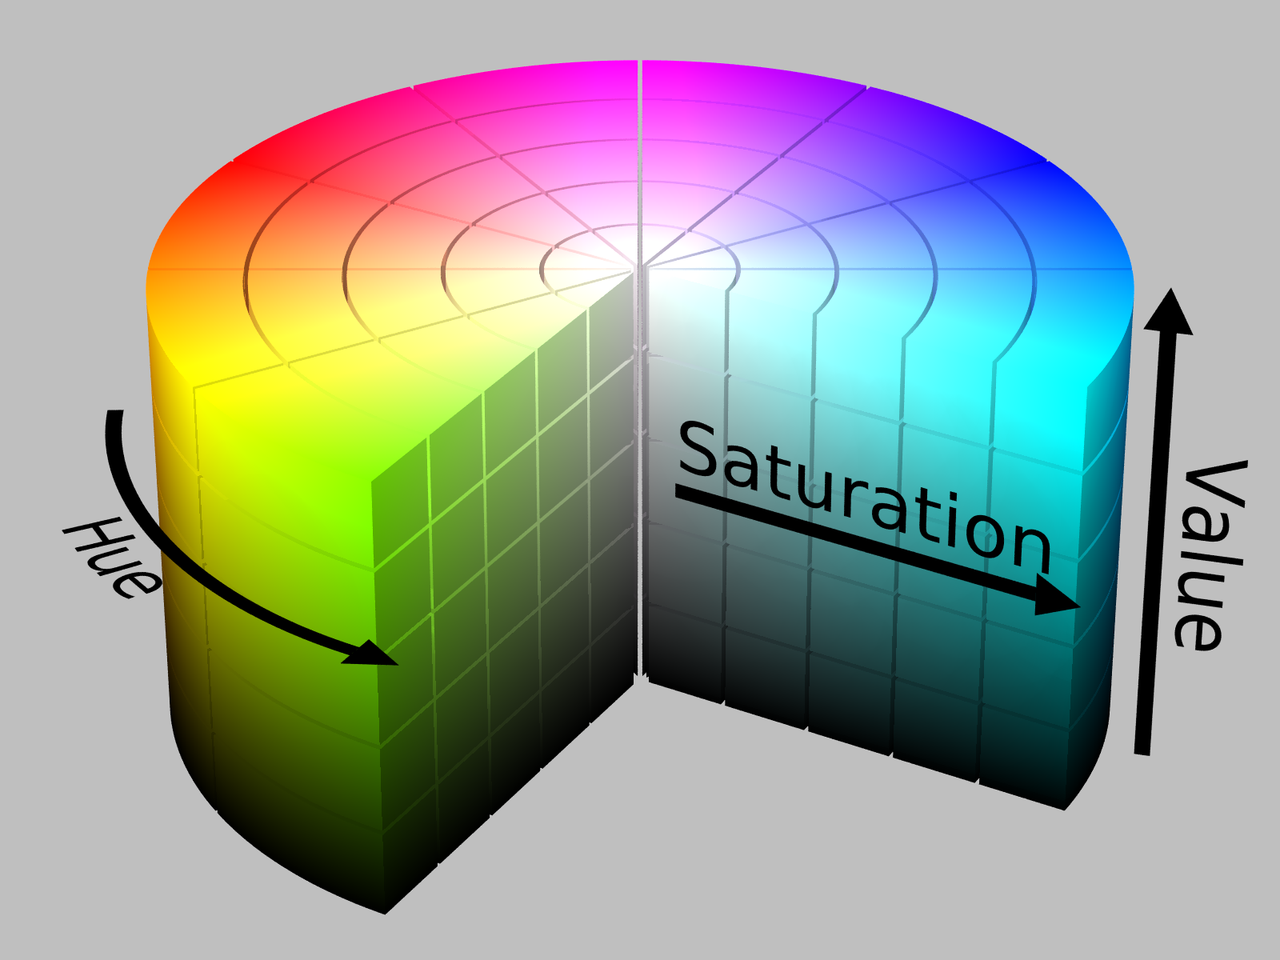
\includegraphics[width=0.3\textwidth]{figures/1280px-HSV_color_solid_cylinder_alpha_lowgamma.png}
\end{figure}

\subsection{Choosing colorspace}
The first challenge we came along was to choose the best colorspace representation in order to overcome the variations in lighting conditions. The dataset we had consisted of RGB images. Unfortunately, it is unfeasible to use the default RGB colorspace for most applications due to influences such as lighting and shadows. We also experimented with normalized RGB colorspace. Theoretically,  normalized RGB would have given us the pure chromaticity values of each object in our field of view, and thus overcoming the problems shadows and lighting conditions can give. However, normalized RGB did not help us achieving a light-invariant color representation, resulting into false positives in color segmentation. HSV was the solution to our problem. HSV is a cylindrical colorspace representation, which contains information about hue, saturation, and value. We found hue to be really informative in order to distinguish easily between colors. Hue defines the pure chromaticity of the color and it is independent of the lighting conditions. In figure~\ref{hsv}, this cylindrical color representation is illustrated. One can see that the hue is represented by the angular dimension in the vertical axis of this cylinder. 


\subsection{Basic Pipeline}
Having described the first basic step of our approach, choosing the proper colorspace for our application, it is time to go deeper into the feature extraction process.
The first step in this process is the image input from the NAO's camera in HSV format. As we said before, images not only contain the important region of the field in which we are interested in, but also some background information which is useless in order to detect field features. This background usually extends above the field horizon and it may become really disturbing in the extraction process. This is the reason why background removal is the first step in our feature extraction scheme. Field lines, goals, ball, and other NAO robots are the features located into the field. In this project, we only took into consideration lines and the goals which are static landmarks, unlike the ball and other robots that are moving as we could not depend on them for self-localization. 

The HSV values are used to binarize the image, with respect to the goals, and with respect to the lines. As we said in the introduction, the field is colored green, both goals are yellow, and lines are white. The next step of the feature extraction is the goal detection, making use of the horizontal and vertical histograms of yellow values. Line detection is followed in order to find a good estimation about the lines detected in our field of view. Having these lines' estimations, we can detect feature on them, using geometric properties. Last step in this process' pipeline is to output all these detected features to the localization core process. We can now enumerate all steps in these pipeline. These steps are:
\begin{enumerate}
\item Input HSV image from camera
\item Background removal
\item Image binarization
\item Line detection
\item Line feature detection
\item Goal detection
\item Output features
\end{enumerate}

\subsection{Image format}
NAO's camera can output images in different colorspace representations and resolutions~\cite{NaoCam}. The images from the dataset we had were in RGB format, and they had QVGA resolution ($320 \times 240$). We wanted to keep a low resolution in order to keep the time complexity of our algorithm feasible for real-time execution. \textbf{Patrick can add some things here as he experimented better with NAO's camera.}

\begin{table}
\begin{center}
\caption{Threshold values used for color segmentation.}
\label{thresholdHSV}
\begin{tabular}{lccc}
\toprule
\multicolumn{4}{c}{\textbf{Threshold}} \\
\cmidrule(r){2-4}
\textbf{Color}   & \textbf{Hue} & \textbf{Saturation} & \textbf{Value} \\
\midrule
Green      & $20 \sim 37$    & $100 \sim 255$    & $100 \sim 255$    \\
Yellow      & $38 \sim 75$    & $50 \sim 255$    & $50 \sim 255$    \\
White     & $0 \sim 255$    & $0 \sim 60$    & $200 \sim 255$    \\
\bottomrule
\end{tabular}
\end{center}
\end{table}

\subsection{Background Removal}
Background removal defines the task of detecting the field's borders in order to exclude uninformative regions in the processing image, saving this way computational cost and helping to subtract only the useful part of the image, which is the one, where we can detect all the features we are interested in. This can be done by a vertical scan of the image and detecting the first green pixel in each column. This method can work efficiently but it is not robust in many cases, as green pixels can be found above the field's horizon as well. Following the same principle in our approach, we consider as background every region in a column before a considerable amount of green pixels, and not just one, which can lead us to faulty decisions about the horizon. We start in each column considering the pixel in the first row as background. Then, during scanning each column, we stop when we find many green continuous pixels and assign as horizon row in this column the first of this sequence of green pixels.  As you can see in table~\ref{thresholdHSV}, green pixels are considered as those which have hue, saturation, and value around these thresholds. Figure~\ref{background}, illustrates the process of background removal. Even though it is not such a sophisticated method, we can see that in this specific example, almost all background above the field's horizon has been removed, helping us in this way to avoid detect false positive features in the background.

\begin{figure*}[t!]
\caption{Background removal process example, original RGB image (left), points indicating the start of the field (middle), regions of interest without background information (right).}
\label{background}
\centering    
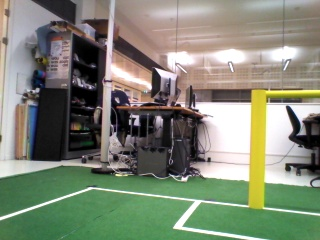
\includegraphics[width=0.3\textwidth]{figures/original.png} \	
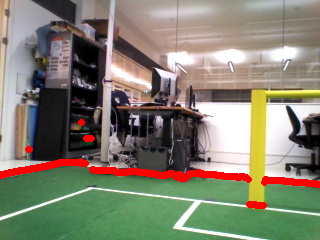
\includegraphics[width=0.3\textwidth]{figures/back.png} \	
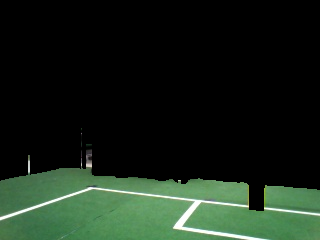
\includegraphics[width=0.3\textwidth]{figures/back_fixed.png}	
\end{figure*}


\subsection{Image Binarization}
In this section, we will talk about another image pre-processing technique which helped our main procedure detect features easier. Image binarization is a process which outputs two binary images, one in respect to the goals, and the other in respect to the field lines. For goal detection, it is natural that we are interested only in yellow areas of the image. The same applies for field lines, we are only interested in green and white areas of it. The main goal of this process is to classify colors according to table~\ref{thresholdHSV}. As we can realize, a simple way to classify colors is used in order to get a binary image, with the interesting part highlighted in each case. For the first case, goals, we are only interested to find yellow, so we output white for each yellow pixel, and black for any other color. For field lines, black for every other than white pixel.

\begin{figure}[h!]
\caption{Binary images in respect to the lines (left),  and to the goal (right), for the example RGB image in Figure~\ref{background}.}
\label{binary}
\centering    
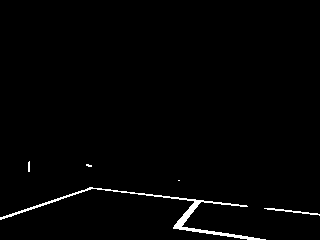
\includegraphics[width=0.22\textwidth]{figures/bin_lines.png} \	
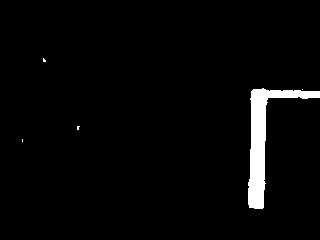
\includegraphics[width=0.22\textwidth]{figures/bin_posts.png} \	
\end{figure}

Figure~\ref{binary}, illustrates the process of image binarization. To add some technical details about the above implementation of image binarization, we can say that the whole process of it is integrated into the background removal procedure which requires only one vertical scan of the input image, and its goal is to minimize the space complexity of the whole feature extraction method, as now we have only to process binary images with only one channel, in contrast to the original 3-channel image.

\subsection{Line Detection}
Before proceeding to the exact procedure about finding goals and line features, it is time to introduce our approach to detect line segments in a binary image like those we presented before in image binarization section.

\subsubsection{Other approaches}
In general, we are interested in finding one line segment for each actual line appearing in the image. Other methods, such as Hough Transformation or Probabilistic Hough Transformation failed to detect these continuous line segments, due to the fact that they applied after edge detection step. Lines in our images consist of line segments which are thicker than one pixel, and when edge detection is applied to those finds edges at both sides of a line. Therefore, both Hough transformations find lines at both sides of an actual line. There were also some other problems with these methods, namely, the big number of detected lines, small line pieces on each actual line, and wrongly connected line segments. Furthermore, the huge number of detected lines, made our efforts to cluster those lines tough.

\subsubsection{Our approach}
As a result, we came up with our own approach of finding line segments in these noisy images. The main idea in this approach is that if we had some points on these actual line segments, we could be able to connect them based on color information, and geometric properties they have. Therefore, the first step of this algorithm, is to generate these points, scanning the picture every $5 \sim 10$ pixels vertically and horizontally. We are only interested in transitions which start from black go white and again black in the end. We store these points as a pixel coordinates $<x,y>$ in a vector. As an illustration, we can see in figure~\ref{points}, where these points are located for the same example input image as before.
\begin{figure}[t!]
\caption{Points produced by black-white-black transitions in the example binary image of figure~\ref{binary}.}
\label{points}
\centering    
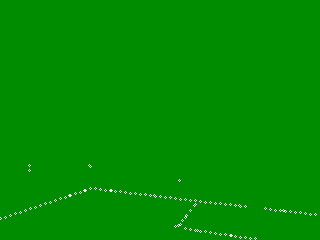
\includegraphics[width=0.4\textwidth]{figures/points.png}
\end{figure}

Once these points have generated, the next step is to connect them in order to form line segments. For the representation of each line segment we hold a queue of points, at each time the line segment is formed by the first and the last point in the queue as starting and ending points. Pushing always the first point of the vector in the queue and deleting it from the vector the same time, we are looking for the closest points (5 points) to this point. From these closest points, we are checking the white ratio between these points and our initial point. Assuming that points from the same line segment, do not have black pixels between them, we connect the closest one with high white ratio, usually $1.0$, and pushing it in the queue of points as the last element and deleting it from the vector. The same procedure continues, but now we are looking to connect the last element on the queue with one from the remaining points in this vector. So, now the question is how are we going to stop connecting points? Considering a line formed by lots of points, these points have to have small distance from the projection point on the line. Based on this idea, we can introduce an error function in order to define when a line starts not to comply with the points consisting it. Assuming a queue of points $Q$, which contains $n$-points, we can say that:
\begin{equation}
Error_Q = \sum_{i=1}^{n}(Eucl.Dist(Q_i, Proj.Point(Q_i,Q)))^2
\end{equation}
This error measure proved to be really informative in our case to understand when a line is starting to consist of points which may not represent the same line segment. When this error becomes larger than a threshold, we store the produced line so far, and we continue with the next point in the vector. To store the line, we first check if there is an already stored line which is an extension of the current line, to find out we measure the error we introduced in equation 1, taking now as line's starting and ending points the points with the largest distance between them. If the error remains small enough, and the closest points of this connection are covered in high white ratio, then we merge these lines which now represent a continuous line.
\begin{algorithm}[t!]
\caption{Line segment detection algorithm}
\label{line}
\begin{algorithmic}[1]
\STATE {\bf Input: }$points, image$
\STATE {\bf Output: }$line$
\STATE{start = points[0]}
\WHILE{points.size() $\neq$ 0}
\STATE{line.push(start)}
\STATE{bestCandidate = findBestCandidate(points, image)}
\STATE{points.erase(bestCandidate)}
\STATE{error = computeError(line, bestCandidate)}
\IF{error < threshold}
\STATE{start = bestCandidate}
\ELSE
\STATE{storeLine(line)}
\STATE{line.clear()}
\ENDIF
\ENDWHILE
\end{algorithmic}
\end{algorithm}
Algorithm~\ref{line}, presents the pseudo-code for the line detection procedure. In line $12$, function $storeLine$, takes as input the produced line, if the line cannot be merged with an already stored line segment, then, it is stored as it is in a vector of lines. In figure~\ref{lines}, we illustrate the produced lines by the above algorithm. We can see the effectiveness of our algorithm to detect lines. A big advantage over the other method we have tried is that we now detect single and continuous lines upon each actual line segment on the field.

\begin{figure}[t!]
\caption{Lines produced by the line segment detection algorithm on the above points generated by the binarized image from the previous figures.}
\label{lines}
\centering    
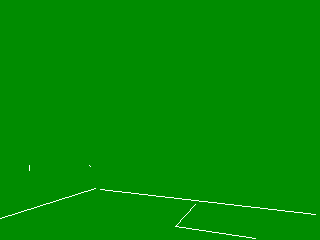
\includegraphics[width=0.4\textwidth]{figures/lines.png}
\end{figure}

\subsection{Line Feature Detection}
Until now, we have talked about, image binarization and how we detect line segments. The next step in our feature extraction procedure, is to identify and extract information about line features. In Robocup SPL field, we can distinguish 4 types of features that can be extracted out of lines. The are three lines intersections types, T, L, X, and a circle in the middle of the field. For the circle or the ellipse detection, as it is seen by the low-height robot's camera, we are going to talk about in a different section. In this section, we are only discussing how we can extract the first three types of intersections.

For this purpose we introduced a confidence measure which is based on geometrical properties of intersections. Given the lines which have been produced by the previous step of the process, we check every possible intersection produced by pairs of lines which have at least $10$ degrees angle difference in order to void find intersections by two continuous lines, and intersection is located within the margins of the image. For each one of these intersections, we compute a confidence measure for T, L, and X types. We can briefly define these measures for the several types:
\begin{itemize}
\item[\textbf{T}]{, the basic idea is that the intersection is located upon the one line of the line-pair, but not close to the line's starting or ending point.}
\item[\textbf{X}]{, intersection must be upon both lines and not close to both lines' starting or ending points. }
\item[\textbf{L}]{, intersection must be close to both lines' starting or ending points.}
\end{itemize}
These measures are computed in a way that an intersection cannot have same confidence for two types. After the computation of the confidence measure for each intersection, we check if there are intersection types which can be combined in one. For example, two T type intersections can form a X type if they are located near and have opposite orientation. Except from the computation of the intersection position and confidence for each type of intersection, we also compute the orientation of each one of them, in order to be feasible for the localization system to acquire more information about the robot's position.

\subsection{Goal Detection}
Last step in the feature extraction process is the detection of the goal. Goal detection is critical for the robot in order to take sensible actions, and due to the fact that is the only easily-distinguishable landmark in the field. Both goals in the Robocup SPL field have a distinct yellow color. We have already discussed how the binary image in respect to the goals is created. Integrated in the same scan of the input image, we compute two different histograms for yellow pixels, one horizontal and one vertical. These histograms are going to help us later in goal detection. We also store points of yellow-green transitions on the same image scanning to estimate like this possible goalposts' bottoms.

Goals consist of two vertical bars and a horizontal attached to the tops of the two vertical bars. So, we can realize that vertical bars are more informative, especially to inform our localization system about the orientation in respect to the goalposts.

\begin{figure*}[t!]
\caption{Goal detection example results( green - left goalpost, red - right goalpost, white - vertical goalpost, blue - horizontal goalpost.}
\label{posts}
\centering    
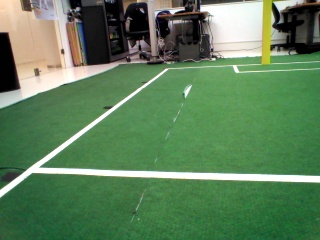
\includegraphics[width=0.3\textwidth]{figures/img_000003.jpg}	
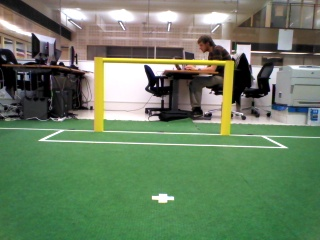
\includegraphics[width=0.3\textwidth]{figures/img_000005.jpg}	
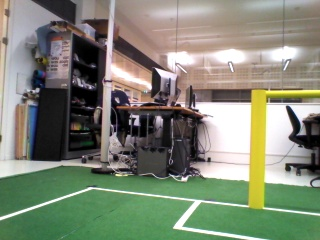
\includegraphics[width=0.3\textwidth]{figures/img_000006.jpg} \\
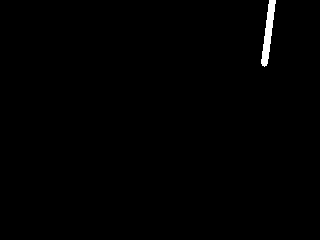
\includegraphics[width=0.3\textwidth]{figures/post3.png}
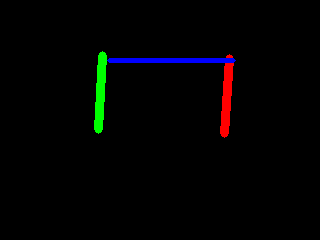
\includegraphics[width=0.3\textwidth]{figures/post5.png}
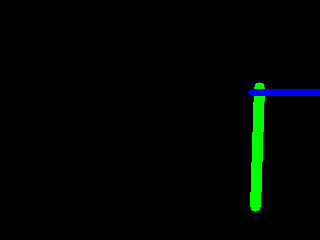
\includegraphics[width=0.3\textwidth]{figures/post6.png}
\end{figure*}

The first step in goal detection process is the use of the horizontal histogram of yellow pixels in combination with the y-positions in where we found yellow-green transitions. Combining this information, we can find the local maxima in the horizontal axis and find the position-s, where goalposts are located. If the maxima of this histogram have values under a certain threshold, the process will not continue for vertical posts detection, as it appears that there is no vertical post. If these values are high enough, and we have two local maxima, we are pretty sure that there are two vertical posts in the image, if there is only one we are looking only for one vertical post. In both cases we scan the image left and right from the maxima and exclude parts of the image which do not contain yellow pixels at all, for computational efficiency.

Next step is the line detection, using the same approach we have discussed earlier, but now generating points only with a vertical scan, as we are only interested in vertical lines. From these vertical lines we choose the best ones in respect to their length, orientation, and with the prior knowledge about possible horizontal positions for the goalposts. These lines will be extended towards the bottom of the goalpost and the top, estimating like this the true height of each goalpost. To estimate the width, we are taking random samples upon the line representing the goalpost and measure with a simple scan the width. The average of all these measurements will be our estimation about its width. We also compute a confidence measure about the bottom of the goalposts, taking the estimated bottom of the representative line and computing the distance from the yellow-green transition we talked earlier. The same procedure is applied for the horizontal goalpost as well. Horizontal goalpost can be very informative in cases that only one vertical goalpost is visible by our agent. The orientation of the Horizontal goalpost can be used in order our agent to distinguish between left and right goalpost. In figure~\ref{posts}, we illustrate the results of the goalpost detection, in three different situations.

\subsection{Ellipse Detection}
The field of the RoboCup Soccer STL league has a circle in the middle with a diameter of 120cm. This is an important feature for the Nao's self-localization as this is the only unique feature on the field. In computer vision, most commonly performed ellipse detection is carried out on binary images from an edge detector. However, in general, ellipse detection does not adress the problem of false positives and false negetives well, especially for partially visible ellipses.

For this project, we chose to implement an ellipse detector based on P{\u{a}}tr{\u{a}}ucean's method~\cite{ED}. We chose this technique for the following reason: It is parameterless and required no special tunining for different scenarios. Most ellipse detectors require as input certain parameters that define the scenary such as a range of expected radii of ellipses, and a minimum distance between two ellipses. This approach aims to be free of critical parameters as much as possible, in order to avoid introducing false negatives. Also, it provides a control over the number of false positives by using \emph{a contrario} validation. The greedy-like candidate selection step implemented by this algorithm ensures a reasonable execution time. The two primary steps in this algorithm are: 

\begin{itemize}
\item Region growing: Pixles with a similar gradient orientation are alligned to form rectangular regions.
\item Region chaining: These detected regions are chained together if they roughly follow some conditions that define ellipses.
\end{itemize}

To tackle the problem of false positives, \emph{a contrario} validation is employed to reject or validate candidate ellipses. The \emph{a contrario} theory employs the non-accidentalness principle (which says that ``we see nothing in noise''). Therefore, as described in \cite{ED}, candidate ellipses that have a higher chance to be observed in noise are discarded. % P: Possible comment I see from Theo/Arnoud is "how is that done?"
However, as can be seen in figure \ref{fig:ED}, even after this step, we still find a number of false positives because small features like penalty X crossings, and resedue background noise often gets classified as small arcs by the ellipse detector. This problem can easily be tackled by filtering the candidate ellipses on their arc lengths and putting a minimum threshold on it.

\begin{figure}
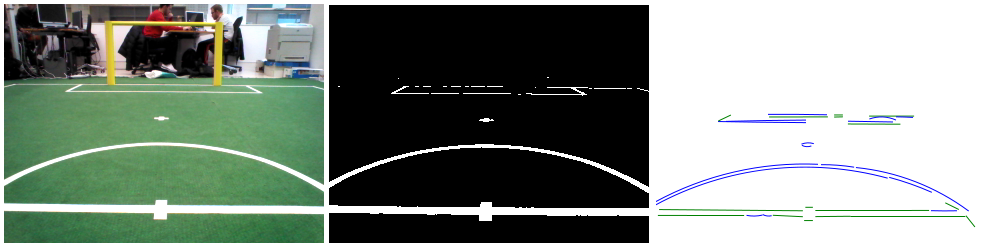
\includegraphics[width = 265px]{figures/ellipseDetection.png}
\caption{Left to right: RGB image obtained from NAO's lower camera, binary image of field lines after background removal, possible ellipses detected (and lines, not considered) }
\label{fig:ED}
\end{figure}

The ellipse detection step can also ensure lesser false positives (and faster computation) during the line feature detections stage if ellipse detection is performed first: If we know with confidence the area that the circumference of the ellipse is covering, we know that line crossings do not exist on it and hence we can mask this area for the line feature detection step.

\subsection{Inverse Perspective Mapping}
Transformation from one projective plane to another can be utilized for generating views of objects different from the camera position. Inverse perspective mapping (IPM) makes use of this. It projects an image on a known plane and gets rid of the perspective effect on objects that are on that plane and produces a distorted view for all others~\cite{IPM2}.

Information like the angle of view (under the horizon) and the distance of objects from camera associate a different information content with each pixel of an image. In fact, the perspective effect must be considered during the processing of images so as to weigh each pixel with respect to its information content. As a counter to this issue, IPM lets us remove the perspective effect and remap the image to a 2D domain, so that the information content is evenly spreadout among all pixels~\cite{IPMWeb}. 

It must be noted that applying the IPM transform requires some camera conditions to be known. These are the camera's height above ground level, its aperture, its tilt with respect to the vertical axis and its resolution. Since this information can be %fairly accurately -- P: not so sure how accurate that is ;)
computed fairly accurately by the Nao through inverse kinemetics, the IPM transformation can be used by it. Thus, assuming that the field in front of the camera is planar, a bird's eye view of the playing field can be obtained.

In the domain of robot soccer, the use of IPM transformation can have a few potential advantages. % P: can we make such a strong statement? do we have the results to claim this? or is it safer to say something like "the advantages can be great, given accurate sensor data"?
Estimation of distance and bearing to a feature point on the field is simplified because now we have a bird's eye view of the field in front of us. Preprocessing steps like background removal is also much easier than on regual camera images because of the fact that always the lower part of the image contains the field. Moreover, IPM also overcomes the problem that the Nao's head can tilt along various axes because this transformation is robust to such viewpoint changes. Lastly, the feature extraction step can itself be made more robust and computationally inexpensive. This is because when viewing the field from a top perspective, all intersecting lines on the field appear to intersect orthogonally and circles retain their shapes. However, one of the main problems we faced while using IPM for feature extraction was that feature points far from the camera appear to get distorted due to the transformation. This causes many false negatives while extracting features. One ad-hoc solution to this problem was transforming the binary image of the lines in the field instead of the raw RGB image. Another problem with using IPM was the difficulty in measuring projected objects such as goal posts on the field. The transformation always streches the goal posts such that their top portions are no longer visible/detectable. Thus, goal post detected continues to rely on frong-facing camera images.

We now briefly explain this transformation\cite{IPM} while not going into the details of its mathematics. In IPM, for a point in the image plane, we trace a ray from this point through the center of projection and towards the horizontal plane, where it results in an intersection. In this way, we find the corrosponding image point.

We first create matrices that contain the $x$ and $y$ locations in the world frame, where the pixels in the bottom portion of the camera image (where we assume we see the field based on the camera's viewing angle, height and aperture) are mapped by using the inverse perspective transformation equations (see figure \ref{fig:IPM}, center). Next, we find the weights needed to create an inverse-perspective-mapped image with evenly spaced pixels by linearly interpolating between intensity/color values in the original image. Finally, we apply the inverse-perspective interpolation mapping to an RBG camera image to get an inverse-perspective-mapped image\cite{IPMCode} (see figure \ref{fig:IPM}, right).

\begin{figure}
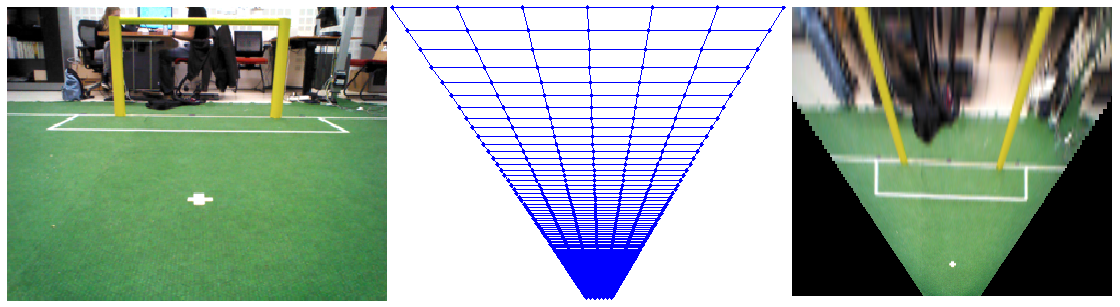
\includegraphics[width = 265px]{figures/imagePixelsMapped.png}
\caption{Left to right: front facing RGB image obtained from NAO's lower camera, map of image pixels to the world frame, bird's eye view obtained after IPM}
\label{fig:IPM}
\end{figure}


\section{Localization}
\label{sec:Localization}
We based our localization module on the Monte Carlo Localization method (MCL). The module has been augmented with several extensions taken from literature. This part of the report describes the standard MCL approach, the models that were used to incorporate incomming sensor information (i.e. odometry and observed visual features in the camera image). We describe how the observed features are associated with the given featuremap of the soccer field. Eventually we elaborate on how the standard approach was improved to overcome well known shortcomings of the usage of particle filters in a robot soccer turnament environment.

We chose to use the MCL as basis for localization of the robot since it is a well known approach, and toroughly researched. It is a multimodal particle based localization method (i.e. it can deal with multiple pose hypothesis at the same time). Since the new environment for 2013 is completely symmetric this is a valuable property. In addition to that, MCL can deal with erroneous sensor information, which is an unavoidable problem in real life applications in robotics. It is able to recover from kidnapping (i.e. repositioning the robot on the field without odometry information). Finally the number of particles can be adjusted. This is usefull, since the NAO robot platform offers only limited computational resources.
\subsection{Monte Carlo Localization}
\label{sec:MCL}
The basic MCL algorithm is depicted in following pseudocode  as described by Fox et al. in \cite{MonteCarloLocalization}:\\


\begin{algorithm}[h!]
\caption{Monte Carlo Localization}
\begin{algorithmic}[1]
\STATE {\bf Input: }$\chi_{t-1}, u_t, z_t,m$
\STATE {\bf Output: }$\chi_t$
\STATE \textbf{monte\_carlo\_localization(}$\chi_{t-1}, u_t, z_t,m$\textbf{)}\\
\STATE $\bar{\chi_t} = \chi_t = \emptyset$
\FOR{$m$=1 to $M$}
\STATE {}$x^{[m]}_t$ = sample\_motion\_model( $u_t$ , $x^{[m]}_{t-1}$ )\;\label{alg:motion_model}
\STATE {}$w^{[m]}_t$ = measurement\_model($z_t$, $x^{[m]}_t$ , $m$)\;\label{alg:measurement_model}
\STATE {}$\bar{\chi} = \bar{\chi} + \langle x^{[m]}_t, w^{[m]}_t \rangle $\;
\ENDFOR
\FOR{$m$=1 to $M$} \label{alg:mcl_resampling}
\STATE draw $i$ with probability $\alpha$  $w^{[i]}_t$\;
\STATE add $x^{[i]}_t $ to $\chi_t$\;
\ENDFOR
\end{algorithmic}
\end{algorithm}


where $m$ denotes the map, $\chi_t$ particles at time $t$, $u_t$ control input / odometry information at time $t$, $z_t$ sensor input (in our case visual features) at time $t$.
\\
In general the MCL consists of three main steps:\\
\textbf{Initialize:} place particles at random
\begin{enumerate}
\item \textbf{process odometry information:} Change particle poses (position and rotation) accordingly. (line : ~\ref{alg:motion_model})
\item \textbf{process visual sensor input (extracted features):} Calculate likelihood of pose hypothesis (particle) and weight particle accordingly. (line : ~\ref{alg:measurement_model})
\item \textbf{resample:} Redraw all particles, place new particles distributed according to the former computed weights, and reset all weights to one. (for loop starting in line :  ~\ref{alg:mcl_resampling} ) %Such that at poses with high likelihood (weight) more particles will end up.
\end{enumerate}
The initialization of particle poses does not necessairily have to be at random, if the initial robot's position is known, or approximately known (e.g. only one side of the field) it is advantageous to sample from this known prior position.\\
Everytime new information is available those three steps can be executed, first process the odometry information, and move all particles accordingly. Since the odometry of robots in the majority of cases incorporates an error, we add additional (gaussian) noise to it. \\
Then we process the visual features, which in our case will be returned from the feature recognition module. Each feature comes with range, bearing and type. In order to compute a likelihood for each pose hypothesis, we need to associate each given feature to a feature of the featuremap. This process is described in detail in the following section. Finally we resample all particles according to the likelihood of each pose hypothesis. Such that at poses that had a high likelihood and thus a high weight, we place more particles. In this step all weights will be reset to one. And we repeat all steps with new incomming information.

\subsection{Sensor Model}
\label{sec:SensorModel}
The feature recognition module returns the range and bearing and type of a feature extracted from the image feed of the NAO robot (an elaborate description of the methods used can be found in section~\ref{sec:FeatureExtraction}). Currently L-crossings, T-crossings and X-crossings and the the bottom of the goal posts can be processed (it is possible to incorporate more types of features, e.g. lines, or the middle circle). These features occure multiple times in the map, it is not possible to distinguish between different features of the same type a priori. For the Monte Carlo Method to work, we need to associate one feature to a feature on our feature map of the soccer field. To determine which observed feature will be associated with which map feature, we compute the observed feature position according to our current pose hypothesis to map space (assuming that we are positioned in the particle position, whose weight we want to compute), then choose to associate it with the feature in the feature map which is closest:
\[\underset{j}{\operatorname{argmin}}  (\sqrt{(m_{j,x} - f_x)^2 + (m_{j,y} - f_y)^2})   \] 
where $f$ is the feature observed, $f_x$ and $f_y$ the feature position and $m_{j,x}$ and $m_{j,y}$ the position of feature $j$ in the featuremap with the same type as observed feature $f$. 

(This simple model was chosen due to time constraints. More elaborate models are possible, e.g. aggregate two or more features and compute correspondence values for those "feature patterns"). To compute the final likelihood, we calculate the range and bearing of the featuremap feature chosen, according to our pose hypothesis. Again we assume erroneous sensory information. For simplicity we model this error as a gaussian, although the underlying error model could be different. 
The sensory model computes the final likelihood of a pose estimate as described in \cite{ProbabilisticRobotics}:
\[ q = \prod\limits_{i=1}^{N}{ prob(r^i  - \hat{r}^j,\sigma_r) * prob(\phi^i - \hat{\phi}^j ,\sigma_{\phi}) * prob(s^i - \hat{s}^j ,\sigma_s)  }  \]
where q is our final likelihood estimate for a certain pose hypothesis, i = 1 .. N the number of features observed in current image of the camera, $ r^i $ the range of the observed feature i, $\hat{r}^j$ the computed range of the feature j in the feature map associated with the observed feature according to the current pose hypothesis, $prob(r^i - \hat{r}^j,\sigma_r)$ denotes the probability of value $r^i - \hat{r}^j$ in a zero mean gaussian with variance $\sigma_r$. $prob(\phi^i - \hat{\phi}^j ,\sigma_{\phi})$ and  $prob(s^i - \hat{s}^j ,\sigma_s)$ denote the probability of a zero mean gaussians for difference in bearing of observed feature $\phi^i$ and bearing of associated map feature $\phi^j$ and probability of $s^i - \hat{s}^j$ on a zero mean gaussian with variance $\sigma_s$ for the difference in certainty of having chosen the right association of feature on the map and observed feature accordingly.


\subsection{Odometry Model}
\label{sec:Odometry}
The odometry model can be either implemented from actual sensor data (through built in accelerometer, or computation of steps taken), or the control input. Since the current implementation was not tested on the NAO robot platform yet, it is still left to further evaluation which input is more advantageous. 
Since both methods incorporate an error, control input through not exactly working motors, or sensor information noise, for each particle we sample from the odometry input with additional noise.
This noise is assumed to be gaussian and independent. At the moment the odometry noise is modelled as error in x and y direction travelled and noise for additional rotation.


\subsection{Augmented Monte Carlo Localization}
\label{sec:AMCL}

Since the standard MCL algorithm described in section ~\ref{sec:MCL} might perform poorly in case of kidnapping.
This is if the confidence of the robot pose is high and it gets replaced from an extrinsic source (e.g. penalty of referee). If the pose confidence is high, the particle density is high around the most probable point in pose space. The robot might get replaced to a pose where no particle is located. It might take a long time till particles will aggregate at the new position. 
A suitable extension to the standard approach is to keep track of the measurement likelihood both in a short term average and a long term average.
If those differ, the robot is capable of detecting a kidnapping situation. New particles can be sampled at random according to the difference of short and long term average. Thus increasing the recover speed after a kidnapping situation as described in \cite{
}:\\



%\For{$m$=1 to $M$ do \label{alg:augmented_resampling}} {
% with probability max\{0.0,1.0 - $w_{fast}/w_{slow}$\} do\label{alg:augmented_resample_start}\\
% \tab add random pose to $\chi_t$\;
% else:\\
% \tab draw $i \in \{1,...N\}$ with probability $\alpha$  $w^{[i]}_t$\;
% \tab add $x^{[i]}_t $ to $\chi_t$ \label{alg:augmented_resample_end}\;}
%  \KwResult{ $\chi_t$ }
\begin{algorithm}[h!]
\caption{Augmented Monte Carlo Localization as depicted in \cite{ProbabilisticRobotics}}
\begin{algorithmic}[1]
\STATE {\bf Input: }$\chi_{t-1}, u_t, z_t,m$
\STATE {\bf Output: }$\chi_t$
\STATE \textbf{augmented\_monte\_carlo\_localization(}$\chi_{t-1}, u_t, z_t,m$\textbf{)}
\STATE static $w_{slow}$,$ w_{fast}$ \label{alg:augmented1}\;
\STATE $\bar{\chi_t} = \chi_t = \emptyset$\;
\FOR{$m$=1 to $M$}
\STATE $x^{[m]}_t$ = sample\_motion\_model( $u_t$ , $x^{[m]}_{t-1}$ )\;
\STATE $w^{[m]}_t$ = measurement\_model($z_t$, $x^{[m]}_t$ , $m$)\;
\STATE $\bar{\chi_t} = \bar{\chi_t} + \langle x^{[m]}_t, w^{[m]}_t \rangle $\;
\STATE $w_{avg} = w_{avg} + \frac{1}{M} w^{[m]}_t $ \label{alg:augmented2}
\ENDFOR
%\STATE $w_{avg} = w_{avg} + \frac_{1}^{M} w^{[m]}_t $ \label{alg:augmented2}\;
\STATE $w_{slow} = w_{slow} + \alpha_{slow}(w_{avg} - w_{slow})$ \label{alg:augmented3}\;
\STATE $w_{fast} = w_{fast} + \alpha_{fast}(w_{avg} - w_{fast})$ \label{alg:augmented4}\;

\FOR{$m$=1 to $M$ \label{alg:augmented_resampling}}
\STATE \textbf{with} probability max\{0.0, 1.0 - $w_{fast}/w_{slow}$\} \textbf{do}
\STATE \tab add random pose to $\chi_t$
\STATE \textbf{else}
\STATE \tab draw $i\in{1,..,N}$ with probability $\alpha$  $w^{[i]}_t$\;
\STATE \tab add $x^{[i]}_t $ to $\chi_t$\;
\STATE \textbf{end with}
\ENDFOR
\end{algorithmic}
\end{algorithm}


To incorporate the long and short term average we change the basic algorithm described in section ~\ref{sec:MCL} as follows:\\
We define the long and short term average in line ~\ref{alg:augmented1}, insert the computation of the current weight average in line ~\ref{alg:augmented2}, then update $w_{slow}$ and $w_{fast}$ in lines ~\ref{alg:augmented3} and ~\ref{alg:augmented4}. With $\alpha_{fast}$ and $\alpha_{slow}$ being the decay rates, where $0<=\alpha_{slow}<<\alpha_{fast}$. Finally we sample particles at random with probability $max\{0.0,1.0-w_{fast}/w_{slow}\}$ and otherwise according to the particle weights computed in the measurement step, as before.
This is called Augmented Monte Carlo Localization (AMCL).
%pseudocode
\subsection{Resetting Sensor Model}
\label{sec:Reset}
Now the robot is to a certain extend able to detect a kidnapping situation (this might take several iterations of the AMCL till the long and short term average differ sufficiently), and injects particles at random. 
In the case of injecting particles totally at random, the localization module is subject to pure chance to sample particles near to the actual position. We can speed up the process in case we have observed visual features. E.g. if we see both goal posts, it is highly unlikely that we are in a position from where we actually cant see any goal.
In this case it is possible to sample from the visual sensor information instead of totally at random a similar method  was originally proposed by Lenser and Veloso  in \cite{SensorResetting}. In our implementation we sample from one feature at random with added gaussian noise in range and bearing. Since we have several features of the same type in the feature map, again we choose one at random for each sample we want to resample. This will result in several circles around all features on the feature map of the type of chosen visual feature to sample from. Due to time constraints, we only chose one observed feature to sample from.
It might increase the recovering speed after a case of kidnapping, to sample from the pose probability distribution of several features (we can reduce the sample space from several circles around the features in the feature map to several points, if we observe and take into account two visible features).


\subsection{Resampling method}
As described by Thrun et al. in \cite{ProbabilisticRobotics} resampling using a random number leads to loss of variance. (e.g. a robot with no perception, after a sufficient amount of resampling steps would only remain with one position hypothesis. Since if sampling with a random number for each particle might lead to the loss of one hypothesis, if two particles are resampled at the same pose).
The following pseudocode depicts low variance resampling:\\
%\begin{algorithm}[H]
% \SetAlgoLined
% \KwData{$\chi_{t},W_t $}
% \textbf{low\_variance\_resampling(}$\chi_{t},W_t$\textbf{)}\\
% $\bar{\chi_t} =  \emptyset$\;
% r = rand(0;$M^{-1}$)\label{alg:resampling_rand}\;
% c = $w^{[1]}_t$\;
% i=1\;
%  \For{$m$=1 to $M$ }{
%  U = r + ($m$-1)* $M^{-1}$\label{alg:stepsize}\;
%  \While{U $>$ c}{
%  i = i + 1\;
%  c = c + $w^{[i]}_t$ \;
%  }
%  add $x^{[i]}_t$ to $\bar{\chi_t}$\;
%  }
%  \KwResult{ $\bar{\chi_t}$ }
% \caption{Low variance resampling as described in \cite{ProbabilisticRobotics}}
%\end{algorithm}
\begin{algorithm}[h!]
\caption{Low variance resampling}
\begin{algorithmic}[1]
\STATE {\bf Input: }$\chi_{t},W_t $
\STATE {\bf Output: }$\bar{\chi_t}$
\STATE \textbf{low\_variance\_resampling(}$\chi_{t},W_t$\textbf{)}\\
\STATE  $\bar{\chi_t} =  \emptyset$
\STATE r = rand(0;$M^{-1}$)\label{alg:resampling_rand}
\STATE c = $w^{[1]}_t$
\STATE  i=1
\FOR{$m$=1 to $M$ }
\STATE U = r + ($m$-1)* $M^{-1}$\label{alg:stepsize}
\WHILE{U $>$ c}
\STATE i = i + 1\;
\STATE c = c + $w^{[i]}_t$
\ENDWHILE
\STATE  add $x^{[i]}_t$ to $\bar{\chi_t}$
\ENDFOR
\end{algorithmic}
\end{algorithm}

Where $X_t$ particles with weights $W_t$ at time $t$, and $M$ the number of particles.
This method creates only one random number, and adds a fixed step size iteratively to a "pointer" (U).
In addition to that we keep track of the sum of particle weights such that, for every step we sample one particle. The particle will be sampled with pose values of particle which "weight bin" (c) the "pointer" is currently pointing. 
This method ensures the systematical coverage of the sample space, and no samples are lost.
We additionaly changed the algorithm slightly, instead of drawing a random number between 0 and $M^{-1}$ (line ~\ref{alg:resampling_rand}) we compute the average particle weight beforhand. This also applies for adding stepsize in line ~\ref{alg:stepsize}, we add the average particle weight instead of $M^{-1}$. This is done to evade complications in case the assignment of particle weights in previous steps is not totally statistically sound.

\subsection{Visualization}
For debugging purposes we developed a simple visualizing modules built on basis of openvc\footnote{\texttt{http://opencv.org/}}. This module reads the parameters of the football field from a parameter file, and can draw the particles, the pose hypothesis of the AMCL. It prvoed to be very usefull, and might be used for future projects.\footnote{The code can be accessed at: \texttt{\url{https://github.com/pkok/Robolab/tree/master/NaoLeague/LocationVisualizer}}}

\section{Evaluation}
\label{sec:Evaluation}

\section{Discussion}
\label{sec:Discussion}
\textbf{???}

However, due to time constraints, the described and implemented parts of the system were only compiled and tested on standard computer hard- and software. The code still has to be tested on the limited resources of the NAO robot.

\subsection{Feature detection}
All tests of the feature recognition were conducted on still images, taken from the NAO's bottom camera. The images of a moving robot will contain a considerable amount of blur, which might require additional tricks to make the whole system robust enough in an actual soccer game, e.g., only classify detected features if they can be observed in a sufficient number of frames.

The existence of other robots on the field will increase the number of false positives the feature recognition will detect.

While the feature extraction works very fast on standard computer hardware, it might be desirable to optimize these routines. For example, one could use the output of the localization module for searching for features at more specific areas of the camera image.  This more educated approach could speed up the feature extraction, as this can be used to eliminate the currently used brute force for checking every pixel.  This might be realized by using the optical flow in the image, or implementing a different tracking method.

\subsection{Localization}
The Monte Carlo localization has a number of parameters, which influence the performance to a great extend.
Although the algorithm can be adjusted to less processing power platforms by decreasing the number of particles, there might be some space to decrease the computational costs by tweaking the code.
Besides that, both the feature recognition and localization do not have to be executed for every new frame. It might be beneficial to postpone computation of features and location updates if the robot does not move, or the computational resources have to be used for other computations.

The localization can be improved performance-wise as well.  We now have implemented an augmented Monte Carlo localization algorithm, which can easily be confused about on which of the two symmetrical halves you are.  For example, B-Human~\cite{TeamReportB-Human} models only half of the field explicitly.  The other half is modeled by using filters that keeps track of the likelihood ${\cal L}$ that this robot is on a certain field half.  By implicit modeling of the second half of the symmetrical field, each particle is twice represented with likelihood ${\cal L}$ to be on one side of the field, and $1 - {\cal L}$ to be on the other half.  On the other hand, rUNSWift does not use a particle filter at all; since 2011 they have been ``experimenting with multi-robot-multi-modal Kalman filtering and researching the application of loopy belief revision to achieve similar benefits, but more efficiently, with larger teams''~\cite{rUNSWift-TD-11}.  Several teams are using self-detected visual features as another source of information for the localization algorithm~\cite{sturm2006msc,Cuauhpipiltin-TD12}.

Another method one could experiment with is triangulation by audio signals.  When at least two NAOs are quite sure about their position, the first could send out an audio signal, which robots unsure about their position will listen to.  The sender will also announce its estimated location over WiFi. Other robots which are certain about their position can do something similar, so that the uncertain robot can estimate its position through triangulation from the bearings.  However, this does rely heavily upon the precision with which the NAO can detect te bearing of the sound.


\section{Conclusion}
\label{sec:Conclusion}


\printbibliography



\end{document}
